\documentclass{article}
\usepackage{amsmath}


%encoding
%--------------------------------------

%----------------------------
\usepackage{microtype}
%\usepackage{fourier}

\usepackage[utf8]{inputenc}
\usepackage[T1]{fontenc}
\usepackage{lmodern}

%units
%--------------------------------------
\usepackage{siunitx}
\usepackage{verbatim}
%drawing
%------------------------------------
\usepackage{tikz} % To generate the plot from csv
\usepackage{pgfplots}
\usepackage{pgfplotstable}
\usepackage{caption}
\usepackage{color, colortbl}
\usepackage{tabularx}
\usepackage{setspace}
\usepackage{mhchem}
\renewcommand{\familydefault}{\sfdefault}
\definecolor{LightCyan}{rgb}{0.88,1,1}
\usetikzlibrary{datavisualization}
\pgfplotsset{compat=newest} % Allows to place the legend below plot
\usepgfplotslibrary{units} % Allows to enter the units nicely
\usepackage{overcite}
\renewcommand\citeform[1]{[#1]}

\sisetup{
  round-mode          = places,
  round-precision     = 2,
  inter-unit-product =\ensuremath{{}\cdot{}}
}

%\usetikzlibrary{arrows, positioning, calc, datavisualization}

\pgfplotsset{
  standard/.style={
    axis x line=bottom,
    axis y line=middle,
  }
}
\usepackage{url}

\begin{document}
%\begin{luacode*}
function string:split(sep)
        local sep, fields = sep or "%s", {}
        local pattern = string.format("([^%s]+)", sep)
        self:gsub(pattern, function(c) fields[#fields+1] = c end)
        return fields
end

function printHyperbola()
    local lines={}

    for line in io.lines("dampf.csv") do
            table.insert(lines, line)
    end
    tex.sprint("\\addplot[color=black] coordinates{")

    for i=2,#lines do
        local a=lines[i]:split()
        tex.sprint("("..a[1]..","..a[2]..")")
    end
     tex.sprint("};")
    tex.sprint("\\addplot[color=blue] coordinates{")

    for i=2,#lines do
        local a=lines[i]:split()
        tex.sprint("("..a[1]..","..a[3]..")")
    end
     tex.sprint("};")

end
\end{luacode*}
%\begin{figure}
\centering
     \begin{tikzpicture}
            \begin{axis}[standard,xlabel=Temperatur,ylabel=Druck]
                \directlua{printHyperbola()}
            \end{axis}
        \end{tikzpicture}
     \end{figure}

\noindent
\begin{onehalfspace}

\section{Ziel des Versuches}
In einer Hydrogencarbonat/Carbonat-Pufferlösung soll die Absorptionsrate für die \ce{CO_2} -
Absorption gemessen werden. Durch Arsenoxid wird die Reaktion katalysiert. Die
Phasengrenzfläche $A$ und die Geschwindigkeitskonstante \ce{k_{kat}} der Reaktion werden ermittelt.
\section{Versuchsdurchführung}
Zuerst wurde eine Stammlösung von 150 mg \ce{As_4O_6} in 300 \si{\milli\liter} 0.5 M \ce{K_2CO_3} -Lösung hergestellt.
Daraus wurden drei weitere Lösungen á 400 mL angesetzt. Die Zusammensetzungen der
Lösungen befinden sich in Tabelle 1. Die Pufferlösung wurde in eine Rührzelle überführt und für ca. 8 Minuten evakuiert. Anschließend wurde unter Rühren Kohlenstoffdioxid über einen Gasballon zugeführt. Über
einen Seifenblasenströmungsmesser wurde die Zufuhrgeschwindigkeit für 20 Minuten
gemessen.
\section{Messwerte}
\text{Konzentration $c(As_4O_6) = 0$ \si{\milli\mol\per\liter}}
% subsection subsection_name (end)
\begin{table}[ht!]
  \centering
 \begin{tabularx}{\textwidth}{XXXX}
$c_{kat}$ [\si{\milli\mol\per\liter}] & \ce{V_{Stamm}} [\si{\milli\liter}]  & \ce{V_{\ce{K_2O_3}}} [\si{\milli\liter}] & \ce{V_{\ce{NaHCO_3}}} [\si{\milli\liter}]  \\
\hline
\rowcolor{LightCyan}
0  & 0 & 200 & 200\\
132.6  & 100 & 100 & 200\\
\rowcolor{LightCyan}
265.3 & 200 & 0 & 200\\
\end{tabularx}
  \caption{Herstellungen der Messlösungen}
\end{table}
Die Pufferlösung wurde in eine Rührzelle überführt und für ca. 8 Minuten evakuiert.
Anschließend wurde unter Rühren Kohlenstoffdioxid über einen Gasballon zugeführt. Über
einen Seifenblasenströmungsmesser wurde die Zufuhrgeschwindigkeit für 20 Minuten
gemessen.

\section{Auswertung}

\begin{table}[!htbp]
\parbox{.45\linewidth}{
\centering

\begin{tabular}{rcc}
\hline
 $t_0$ & $t_5$  & $t_{10}$ \\
\hline
40 & 18 & 38 \\
130 & 19 & 41 \\
230 & 23 & 48 \\
300 & 23 & 49 \\
380 & 25 & 50 \\
450 & 25 & 51 \\
540 & 25 & 51 \\
600 & 25 & 51 \\
680 & 24 & 49 \\
760 & 26 & 52 \\
840 & 27 & 51 \\
910 & 26 & 53 \\
1020 & 25 & 52 \\
1080 & 26 & 50 \\
1160 & 27 & 55 \\
\hline
\end{tabular}
\caption{$c_{kat} = 200$ \si{\milli\gram\per\mol}}
}
\hfill
\parbox{.45\linewidth}{
\centering
\begin{tabular}{rcc}
\hline
 $t_0$ & $t_5$  & $t_{10}$ \\
\hline
10 & 19 & 41 \\
70 & 24 & 49 \\
150 & 27 & 52 \\
240 & 26 & 52 \\
310 & 27 & 55 \\
390 & 28 & 56 \\
480 & 26 & 55 \\
550 & 28 & 57 \\
660 & 28 & 55 \\
810 & 29 & 58 \\
900 & 29 & 59 \\
990 & 30 & 59 \\
1080 & 30 & 61  \\
1170 & 30 & 60 \\
\hline
\end{tabular}
\caption{$c_{kat} = 100$ \si{\milli\gram\per\mol}}
}
\end{table}


\begin{table}[!htbp]
\parbox{.45\linewidth}{
\centering

\begin{tabular}{rcc}
\hline
 $t_0$ & $t_5$  & $t_{10}$ \\
\hline
60 & 24 & 51 \\
140 & - & - \\
180 & 29 & - \\
300 & 33 & 66 \\
420 & 33 & 67 \\
510 & - & - \\
570 & 35 & 68 \\
660 & 34 & 70 \\
780 & 35 & 71 \\
870 & 36 & 72 \\
960 & 35 & 71 \\
1050 & 36 & 73 \\
\hline
\end{tabular}
\caption{$c_{kat} = 0$ \si{\milli\gram\per\mol}}
}
\end{table}


\subsection{Ermittlung der Absorptionsrate}
  Das \ce{CO2} in der Lösung geht in zwei Reaktionen ein.\\
 \textbf{[A]} \: \ce{CO2 + OH- -> HCO3^{-}} \\
 \textbf{[B]} \: \ce{CO2 + H2O ->[kat.] HCO3^{-} + H+} \\

Ohne Präzens eines Katalysators überwiegt die Reaktion \textbf{[A]}, 
wird sich allerdings unter Wirkung der Arsenite \ce{AsO3^3-}, \ce{HAsO3^2-},\ce{H2AsO3^-}
die Reaktion \textbf{[B]} durchsetzen. 
\begin{align}
  r_{ges} &= r _a + r _b + r _{kat}\\
  r_{ges} &= k_a \cdot c_{\ce{CO2}} \cdot c_{\ce{OH-}} + k_b \cdot c_{\ce{CO2}} \cdot c_{\ce{H20}} + k_{kat.} \cdot c_{\ce{CO2}} \cdot c_{\ce{H20}} \cdot c_{kat}   
\end{align}

\begin{equation}
  \ce{r_{ges}} = \ce{k _0} + \ce{k_{kat}} \cdot \ce{c_{kat}}
\end{equation}
Um \ce{k_{kat}} zu berechnen muss zuerst die Absorptionsrate von \ce{CO2} \ce{\.{n}_{\ce{CO2}} } berechnet werden.

%\begin{equation}
 % \frac{\ce{\.{n}_{\ce{CO2}} }}/t
%\end{equation}

        
 %t  5 ml
%\begin{align}
%  y & = -1.03 \cdot 10^{-5} x^2 - 1.861 \cdot 10^{-2} x + 1.796 & R^2 = 0.8566 \\
%\end{align}

%              Estimate Std. Error t value Pr(>|t|)    
%(Intercept)  4.547e+01  1.498e+00  30.357 5.86e-12 ***
%t2           2.836e-02  6.219e-03   4.559 0.000817 ***
%I(t2^2)     -1.417e-05  5.129e-06  -2.762 0.018493 *  
%R= 0.7936
%R = 0.8496
%R = 0.9287



\begin{figure}[htbp!]
      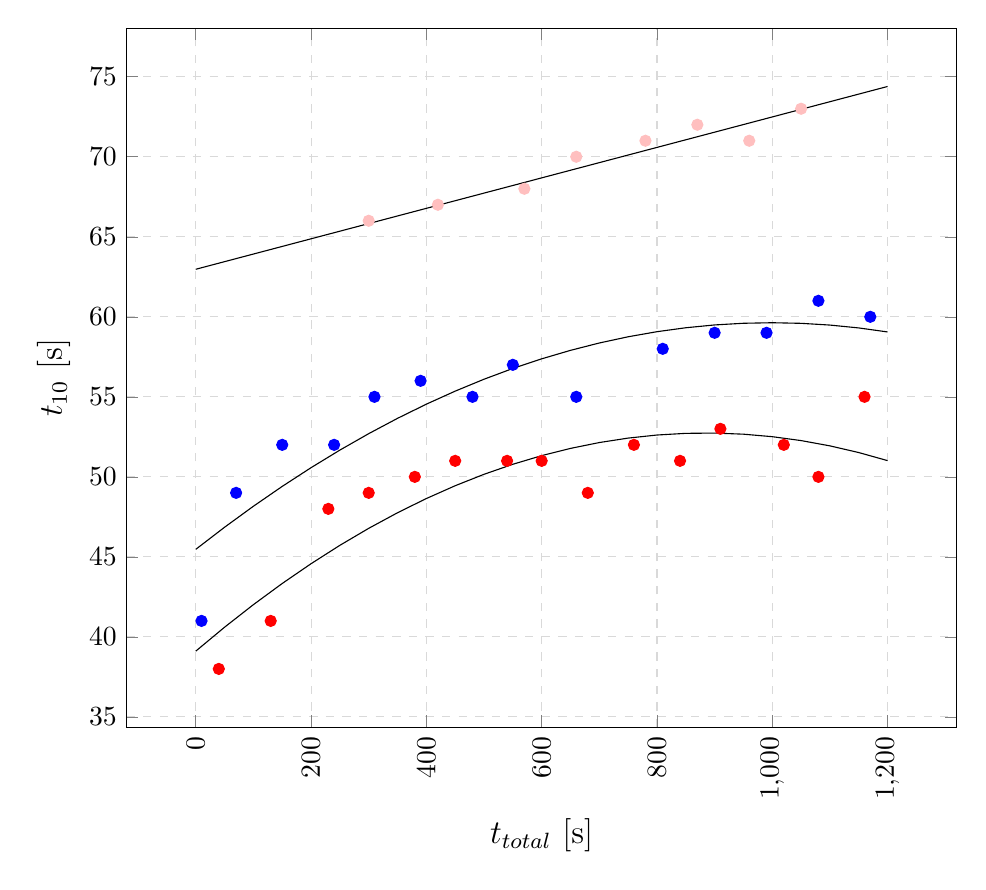
\begin{tikzpicture}
      \begin{axis}[
          width=\linewidth, % Scale the plot to \linewidth
          grid=major,
          grid style={dashed,gray!30},
          ylabel= $t_{10}$, % Set the labels
          xlabel= $t_{total}$,
          xlabel style={font=\large},
          ylabel style={font=\large},
          x unit= \si{\second} , % Set the respective units
          y unit= \si{\second},
          x tick label style={rotate=90,anchor=east}
          ]
\addplot[domain=0:1200]{-1.74e-5*x^(2)+3.08e-2*x+39.11};
\addplot[domain=0:1200]{-1.42e-5*x^(2)+2.836e-2*x+45.47};
\addplot[domain=0:1200]{9.518e-3*x+62.97};

 \addplot[only marks,color=red] table{
40   38
130  41
230  48
300  49
380  50
450  51
540  51
600  51
680  49
760  52
840  51
910  53
1020 52
1080 50
1160 55
    };

 \addplot[only marks,color=blue] table{
10   41
70   49
150  52
240  52
310  55
390  56
480  55
550  57
660  55
810  58
900  59
990  59
1080 61
1170 60
 };

 \addplot[only marks,color=pink] table{
300  66
420  67
570  68
660  70
780  71
870  72
960  71
1050 73
};

\end{axis}
\end{tikzpicture}
\caption*{Abbildung 1.1: Bestimmung von $t_0$ }

\end{figure}

Anhand der Achsenabschnitte sind die \ce{t0}-Werte zu erhalten:

\begin{table}[ht!]
  \centering
 \begin{tabularx}{\textwidth}{XXXX}
\ce{c_{kat}} [\si{\milli\mol\per\liter}] & 0  & 132.6 & 256.3  \\
\hline
\rowcolor{LightCyan}
\ce{t0}  & 62.97 & 45.47 & 39.11\\
\end{tabularx}
  \caption{ Ermittlung von \ce{t0}}
\end{table}

Die Stoffmenge \ce{n_{\ce{CO2}}} lässt sich über das ideale Gesetz berechnen.

\begin{equation}
  \ce{n_{\ce{CO2}}} = \frac{p \cdot V}{R \cdot T} = \frac{101325 \si{\pascal} \cdot 10^{-5} \cdot \si{\cubic\meter}}{ 8.314 \si{\joule\per\mol\per\kelvin} \cdot 298 \si{\kelvin}} = 0.409 \si{\milli\mol}
\end{equation}
wobei das Volumen \ce{V_{\ce{CO2}}} 10 \si{\milli\liter} ist.

\begin{table}[ht!]
  \centering
 \begin{tabularx}{\textwidth}{XXX}
\ce{c_{kat}} [\si{\milli\mol\per\liter}] & \ce{t0} [\si{\second}]  & \ce{\.{n}_{\ce{CO2}}}  [\si{\milli\mol\per\second}]  \\
\hline
\rowcolor{LightCyan}
0  & 62.97 & 0.006495 \\
132.6  & 45.47 & 0.008994 \\
256.3   &  39.11 & 0.01046 \\
\end{tabularx}
  \caption{ Ermittlung von \ce{\.{n}_{\ce{CO2}}} }
\end{table}

\subsection{ Ermittlung von \ce{k_{kat}}}

Anhand der Gleichung: 
\begin{equation}
  \ce{\dot{n}_{\ce{CO2}}^2} = \ce{k0A^2D^L c_{\ce{CO2}^{i^2}} + k_{kat} c_{kat} A^2 D^L c_{\ce{CO2}^{i^2}}}
\end{equation}

Wird nun \ce{\.{n}_{\ce{CO2}}^2} gegen \ce{c_{kat}} aufgetragen ergibt sich eine gerade mit Steigung.
\begin{equation}
  tan \gamma = k _{kat} A^2 D^L c _A^i
\end{equation}

Somit ergibt sich:
\begin{table}[ht!]
  \centering
 \begin{tabularx}{\textwidth}{XXXX}
\ce{c_{kat}} [\si{\mol\per\cubic\centi\meter}] & \ce{t0} [\si{\second}]  & \ce{\.{n}_{\ce{CO2}}}  [\si{\mol\per\second}] & \ce{\.{n}_{\ce{CO2}}^2}  [\si{\square\mol\per\square\second}]  \\
\hline
0  & 62.97 & \num{6.495e-6} & \num{42.185e-12}  \\
\num{3.03e-7}  & 45.47 & \num{8.994e-6} & \num{80.89e-12} \\
\num{6.06e-7}  &  39.11 & \num{10.46e-6} & \num{109.4e-12} \\
\end{tabularx}
  \caption{ Ermittlung von \ce{\.{n}_{\ce{CO2}}} }
\end{table}

\begin{figure}[htbp!]
      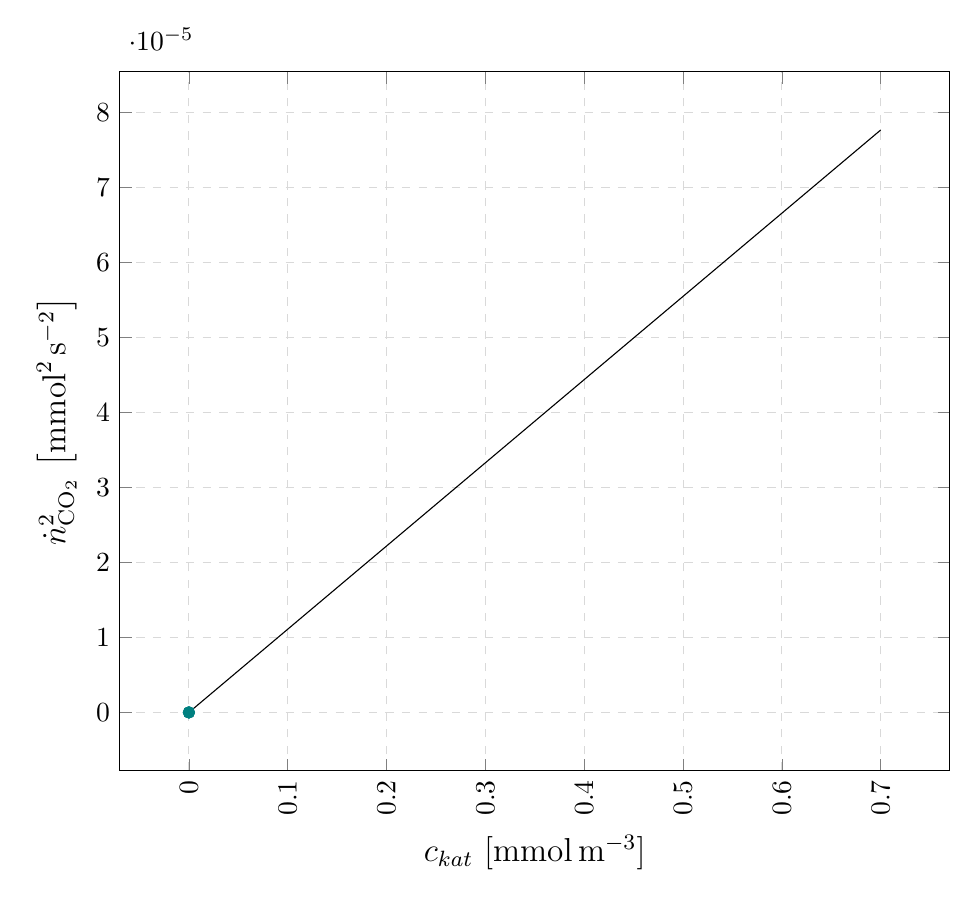
\begin{tikzpicture}
      \begin{axis}[
          width=\linewidth, % Scale the plot to \linewidth
          grid=major,
          grid style={dashed,gray!30},
          ylabel= $\dot{n}_{\ce{CO2}}^2$, % Set the labels
          xlabel= $c_{kat}$,
          xlabel style={font=\large},
          ylabel style={font=\large},
          x unit= \si{\milli\mol\per\cubic\meter} , % Set the respective units
          y unit= \si{\square\milli\mol\per\square\second},
          x tick label style={rotate=90,anchor=east}
          ]
 \addplot[only marks,color=teal] table{
0     42.185e-12
3.03e-7 80.89e-12
6.06e-7 109.4e-12
};
\addplot[domain=0:0.7]{1.109e-4*x+4.388e-11};
\end{axis}
\end{tikzpicture}
\caption*{Abbildung 1.1: Bestimmung von $t_0$ }

\end{figure}
%Multiple R-squared:  0.9924,    Adjusted R-squared:  0.9848 
$tan \gamma$ entspricht der Steigung, 
\begin{equation}
  k_{cat} = \frac{tan \gamma}{D^L \cdot A^2 \cdot c_{\ce{CO2}^{i^2}}} = \frac{\num{1.109e-10}}{D^L \cdot A^2 \cdot c_{\ce{CO2}^{i^2}}}
\end{equation}

Zur Ermmitlung der \ce{k_{cat}} muss die Phasengrenzfläche \ce{A} noch bestimmt werden. 

\begin{align}
  A &= \sqrt{\frac{b}{k_0 \cdot D^L \cdot c_A^i}} \\
    &= \sqrt{\frac{\SI{4.388e-11}{\square\mol\per\square\second}}{\SI{0.86}{\per\second} \cdot \SI{1.6e-5}{\square\centi\meter\per\second} \cdot \SI{1.925e-5}{\mol\per\cubic\centi\meter} }}\\
\end{align}

Durch Einsetzen der Phasengrenzfläche \ce{A}, \ce{D^L} = \SI{1.6e-5}{\square\centi\meter\per\second} 
und \ce{c_A^i} = \SI{1.925e-5}{\mol\per\cubic\centi\meter} in die Gleichung (7) ergibt sich:

\begin{equation}
 \frac{\num{1.109e-4}}{\SI{1.6e-5}{\square\centi\meter\per\second} \cdot  \cdot \SI{3.706e-10}{\square\mol\per\centi\meter\tothe{6}} }
\end{equation}
\begin{equation}
  A = 128.56 \si{\square\centi\meter}
\end{equation}
\begin{thebibliography}{}
\bibitem{crc1}
D. R. Lide, \textit{CRC Handbook of Chemistry and Physics}, 88. Aufl., CRC Press, New York \textbf{2007}, S. 888.
\bibitem{crc2}
D. R. Lide, \textit{CRC Handbook of Chemistry and Physics}, 88. Aufl., CRC Press, New York \textbf{2007}, S. 1069.
\bibitem{crc3}
\url{http://webbook.nist.gov/chemistry/fluid/}
\bibitem{skript1}
A. Brehm, \textit{Praktikumskript Wärmeübertragung}, Oldenburg, \textbf{2014},  S. 14.
\end{thebibliography}
\end{onehalfspace}

\end{document}
